%%% Object Grasping Dataset 

\subsubsection{Object Grasping Dataset}
\label{sec:ObjectGraspingDataset}

In this section we present an object grasping dataset, collected at the University of Pisa, to be used within the PaCMan project as a tool to perform high level planning and grasping.
The goal of this dataset is to provide a grasp database for each object so that the relative pose between object and hand is always known during the grasp. This information can be later 
exploited to reproduce the grasp autonomously. 
The dataset is composed by sub-datasets, each one containing a series of grasps performed on a kitchen environment object. The grasps are performed by a human operator, wearing
a motorized handle on his right arm, which supports and operates the Pisa/IIT SoftHand, the operator drives the SoftHand to grasp the object put on a table. 
\begin{figure}[!tb]
  \centering
  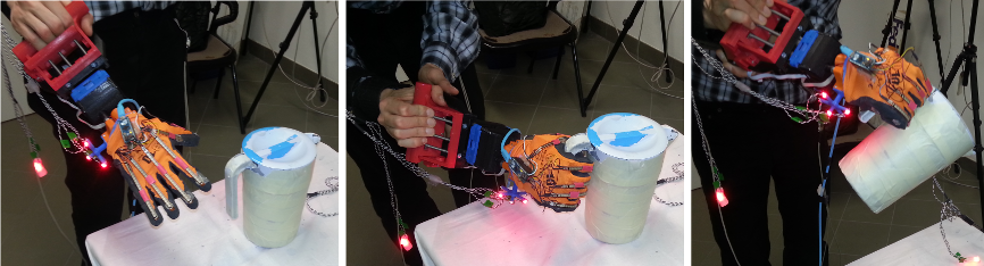
\includegraphics[width=0.955\textwidth]{GRP_subdb1.png}
  \caption{Pictures taken during the recording of the jug sub-dataset. The operator drives the SoftHand towards the object, then grasps and lifts it, while sensor data is being recorded.}
  \label{fig:grasp:subdb1}
\end{figure}
Figure~\ref{fig:grasp:subdb1} show photographs taken during the acquisition of a sub-dataset.
In each sub-dataset several different grasp types were performed, according to the object shape. A goal we kept in mind was to mimic human behaviour in grasping everyday objects, for instance a cup was grasped by the handle, 
by the top without putting fingers inside it or by the sides and so on\ldots
Each grasp recorded is composed by a pre-grasp phase and an actual grasp phase. In the first the operator moves the SoftHand towards the object and starts closing over the designated spot and in the latter the SoftHand 
closes on the object and it is lifted up for a few seconds, then the object is put back on the table and the record stops. The user is able to distinguish between these two phases by reading sensor data: for instance joint positions
of each SoftHand finger is being recorded, so one can notice when the hand starts closing on the object or when it is just moving towards it.
The dataset is then populated by 8-10 seconds long records, each classified in sub-datasets according to the object that is grasped. On each record the user has constant access to relative and/or absolute hand posture, object pose,
hand joints positions and point clouds of the whole scene. In fact the philosophy of the dataset was to collect as much data as possible during the grasp and then give the user the flexibility to chose which data to use for his application.
The remainder of the section describes which hardware was used during records and how it was configured, which software was used and finally a description and usage of data.

\paragraph{(a) Hardware setup used during dataset recording:}
%description of various hardware used
The whole system used to capture grasp recordings is composed by the following subsystems:
\begin{itemize}
  \item PhaseSpace Impulse Motion Tracking System.
  \item Pisa/IIT SoftHand.
  \item Handle for SoftHand.
  \item Flexi Force glove for SoftHand.
  \item Asus Xtion Pro Live.
\end{itemize}

The PhaseSpace Impulse system captures real-time motion by using cameras and LEDs.
The cameras detect the positions of the LEDs, which can be identified via an ID, and transmit the position of each LED in real-time at a frequency of 480Hz.
The main use of this system is to track the position of the SoftHand and the object to be grasped, so that the user has access to these data. 
To accomplish this feature two star-like prints were created to hold five LEDs each, one star was fixed to the SoftHand, the other on the object to be grasped.
Once calibrated the system identifies the two stars and attach a local reference system to them, which they give, respectively, the pose of the SoftHand and the object in space. %maybe explain better
In Figure~\ref{fig:grasp:star} pictures of the stars attached to the object and the SoftHand are visible.
\begin{figure}[b!]
  \centering
  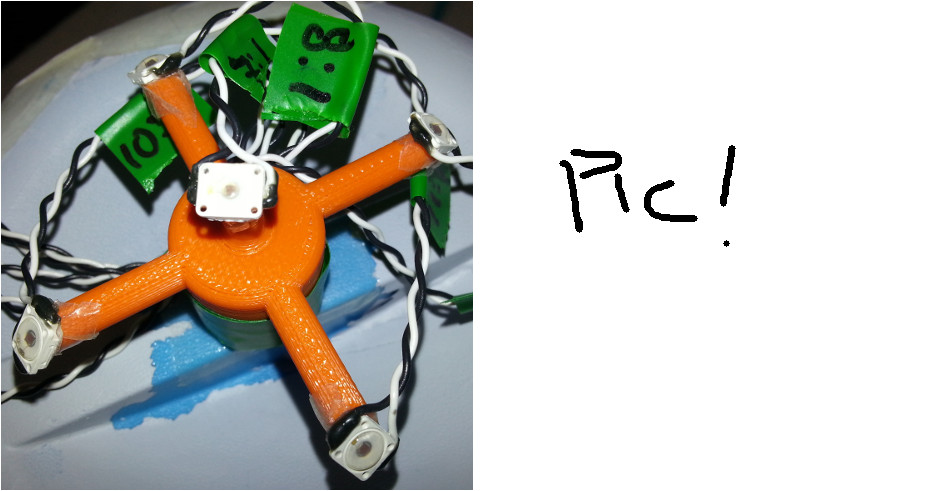
\includegraphics[width=0.95\textwidth]{GRP_star}
  \caption{The star with five LEDs used to track the pose of objects (left). The star used to track the SoftHand (right). The five unique LED IDs and their relative position, identify a local reference system for each star, which are then tracked by the PhaseSpace system.}
  \label{fig:grasp:star}
\end{figure}

The Pisa/IIT SoftHand was dressed with a special glove, called Flexi Force Glove, also designed at the University of Pisa.
Glove readings give a measure of finger bending and consequently joint angle values are estimated to be one third of the finger bending. This is a good approximation considering 
the SoftHand synergies and the type of application. Figure~\ref{fig:grasp:hand_glove} shows the SoftHand with and without the glove.
\begin{figure}[tbh!]
  \centering
  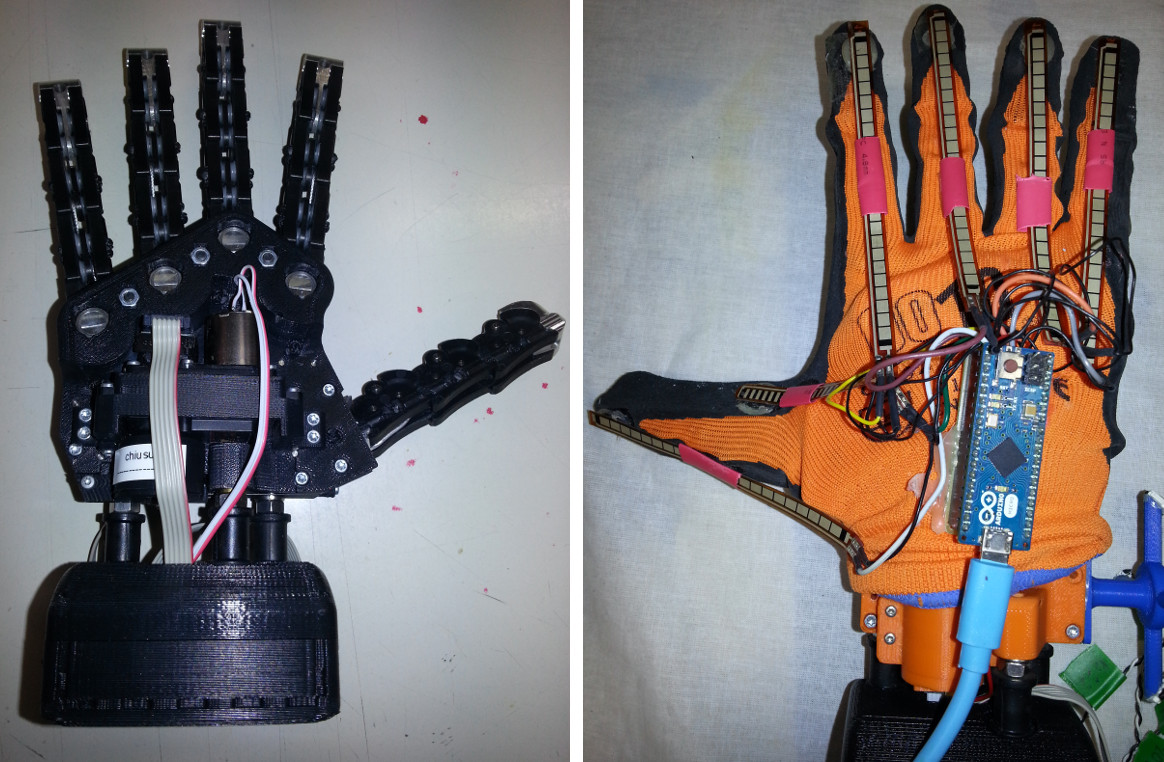
\includegraphics[width=0.95\textwidth]{GRP_hand_glove}
  \caption{The Pisa/IIT SoftHand without the FlexiForce Glove (left) and another one with it (right). Note the sensors alongside the hand fingers that measure the angular displacements.}
  \label{fig:grasp:hand_glove}
\end{figure}

Additionally, to ease the operator in manoeuvring the SoftHand a special support handle was created and used. This device can be attached to the operator's arm so that he can efficiently move and operate the SoftHand, similarly as he would with his own hand.
The handle has a lever to open and close the SoftHand with ease, a photograph of this device is visible in Figure~\ref{fig:grasp:handle}.
\begin{figure}[b!]
  \centering
  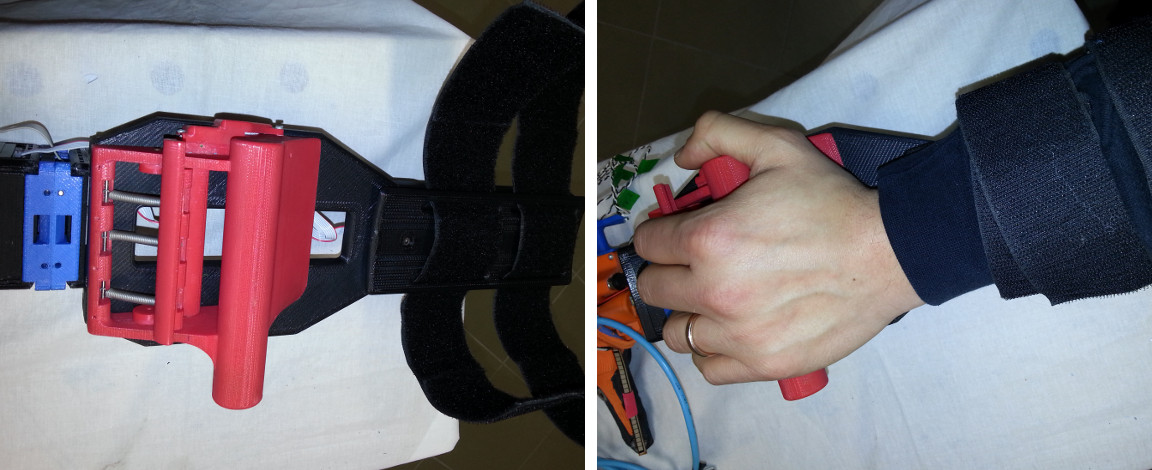
\includegraphics[width=0.95\textwidth]{GRP_handle}
  \caption{The handle for SoftHand without (left) and with (right) the operator's arm. The lever to close the hand is located where the operator's hand should rest.}
  \label{fig:grasp:handle}
\end{figure}

Finally the Asus Xtion Pro Live RGB-D sensor was used to record point clouds and images of the scene while the grasp was recorded. This not only provides the user with more visual feedback, but it also gives more data that
could be post processed to analyze the grasp in a perceptual sense.
\paragraph{(b) Software setup used during dataset recording:}
%1mention we used ROS to sync various hardware
%2talk about calibration steps, and pose estimation paper
%3link and mention github repository where the software is stored
The software employed was developed under the Robot Operating System (ROS) framework. ROS is an open-source set of software and tools widely used in robotics community,
that provides structured communications between heterogeneous hardware designed for robotics application in general.
For our scenario we needed a common platform to communicate with all the various hardware we used and record meaningful data.
The software is available at \href{https://github.com/CentroEPiaggio/unipi-grasp-datasets/tree/master/scenario1}{our GitHub repository} along with a description of the various packages used and the procedure to replicate the grasp
recordings and playing them back. %put url in bib and url pacman project url
As a brief summary the software employs a communication framework like in Figure.~\ref{fig:grasp:software}, %add pic from tf or draw one
where all devices are configured and calibrated together. 
Calibration steps for the experiment are also described in detail on the project website %bib link
and covers:
\begin{itemize}
  \item Calibration between PhaseSpace system and Asus Xtion.
  \item Calibration between first star and SoftHand.
  \item Calibration between second star and the object to be grasped.
\end{itemize}

The first one has to performed just once at the initial setup phase of the experiment, the second was done by means of geometric transformations: knowing the SoftHand and star cad models and where the latter was fixed on the hand.
The last calibration instead is more involving, since it has to be performed every time a new object is selected for grasping. This calibration is performed by knowing the pose of the second star with respect to the PhaseSpace and the
pose of the object with respect to the Asus camera, now since the two systems are calibrated with each other (from first calibration), the pose of the object with respect to the star is obtained by concatenating known transformations.
The last calibration remains valid until another object is selected or the star is moved.
To obtain the pose of the object with respect to the camera we created a procedure to achieve pose estimation with rgb-d vision.
%brief description of the procedure


\paragraph{(c) Data collection and description:}
%explain exactly what is recorded and bagfiles
%data format: msgs, tfs, pointclouds
\paragraph{(d) Data usage:}
%talk about how to playback (link)
%talk about what we could extract from recordings and possible uses (grasp planning)
\paragraph{(e) Data access methods:}
%where the data is stored and how a user can access it




